\documentclass[tikz,border=10pt]{standalone}
\usetikzlibrary{shapes.geometric, arrows.meta, positioning, calc, fit, backgrounds}

\begin{document}
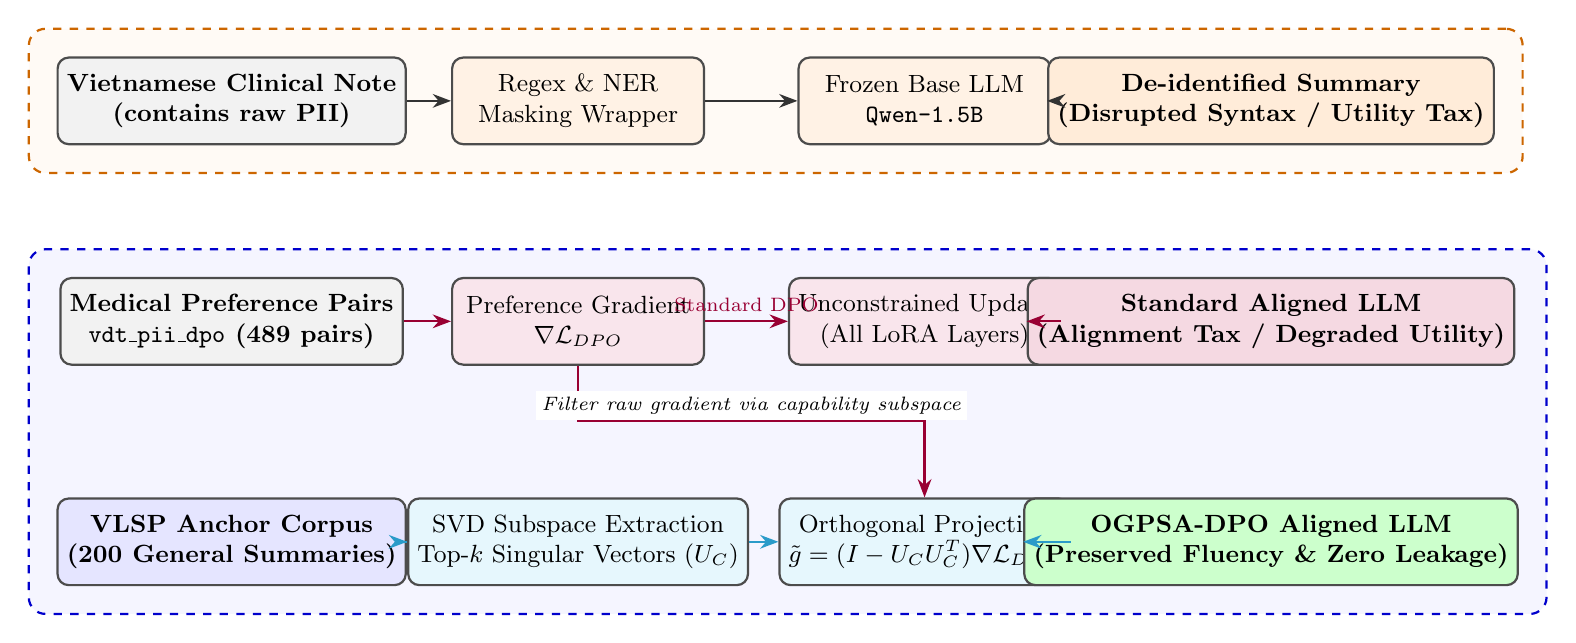
\begin{tikzpicture}[
    box/.style={
        rectangle, 
        draw=black!70, 
        fill=blue!5, 
        thick, 
        rounded corners=4pt, 
        align=center, 
        minimum height=1.1cm, 
        minimum width=3.2cm,
        font=\small
    },
    inputbox/.style={
        box, 
        fill=gray!10, 
        minimum width=3.5cm,
        font=\small\bfseries
    },
    outputbox/.style={
        box, 
        minimum width=3.4cm,
        font=\small\bfseries
    },
    filterbox/.style={
        box, 
        fill=orange!10
    },
    dpobox/.style={
        box, 
        fill=purple!10
    },
    ogpsabox/.style={
        box, 
        fill=cyan!10
    },
    arrow/.style={
        -{Stealth[scale=1.0]}, 
        thick, 
        draw=black!80
    },
    dpoarrow/.style={
        -{Stealth[scale=1.0]}, 
        thick, 
        draw=purple!80!black
    },
    ogpsaarrow/.style={
        -{Stealth[scale=1.0]}, 
        thick, 
        draw=cyan!80!black
    }
]

    % --- PARADIGM 1: EXTRINSIC HEURISTIC DEFENSE (TOP TRACK, Y = 3.6) ---
    \node[inputbox] (note1) at (0, 3.6) {Vietnamese Clinical Note\\(contains raw PII)};
    \node[filterbox] (regex) at (4.4, 3.6) {Regex \& NER\\Masking Wrapper};
    \node[filterbox] (base_llm) at (8.8, 3.6) {Frozen Base LLM\\\texttt{Qwen-1.5B}};
    \node[outputbox, fill=orange!15] (out1) at (13.2, 3.6) {De-identified Summary\\(Disrupted Syntax / Utility Tax)};

    \draw[arrow] (note1) -- (regex);
    \draw[arrow] (regex) -- (base_llm);
    \draw[arrow] (base_llm) -- (out1);

    % --- PARADIGM 2 & 3: INTRINSIC PREFERENCE ALIGNMENT (BOTTOM TRACKS) ---
    % Standard DPO Row (Y = 0.8)
    \node[inputbox] (pref_data) at (0, 0.8) {Medical Preference Pairs\\\texttt{vdt\_pii\_dpo} (489 pairs)};
    \node[dpobox] (dpo_grad) at (4.4, 0.8) {Preference Gradient\\$\nabla \mathcal{L}_{\text{DPO}}$};
    \node[dpobox] (std_update) at (8.8, 0.8) {Unconstrained Update\\(All LoRA Layers)};
    \node[outputbox, fill=purple!15] (out2) at (13.2, 0.8) {Standard Aligned LLM\\(Alignment Tax / Degraded Utility)};

    % OGPSA Row (Y = -2.0)
    \node[inputbox, fill=blue!10] (vlsp_data) at (0, -2.0) {VLSP Anchor Corpus\\(200 General Summaries)};
    \node[ogpsabox] (svd_box) at (4.4, -2.0) {SVD Subspace Extraction\\Top-$k$ Singular Vectors ($U_C$)};
    \node[ogpsabox] (proj_box) at (8.8, -2.0) {Orthogonal Projection\\$\tilde{g} = (I - U_C U_C^T) \nabla \mathcal{L}_{\text{DPO}}$};
    \node[outputbox, fill=green!20] (out3) at (13.2, -2.0) {OGPSA-DPO Aligned LLM\\(Preserved Fluency \& Zero Leakage)};

    % Horizontal Arrows for Intrinsic Alignment
    \draw[dpoarrow] (pref_data) -- (dpo_grad);
    \draw[dpoarrow] (dpo_grad) -- node[above, font=\scriptsize\color{purple!80!black}] {Standard DPO} (std_update);
    \draw[dpoarrow] (std_update) -- (out2);

    \draw[ogpsaarrow] (vlsp_data) -- (svd_box);
    \draw[ogpsaarrow] (svd_box) -- (proj_box);
    \draw[ogpsaarrow] (proj_box) -- (out3);

    % Cross-connection: DPO Gradient into OGPSA Projection Box
    \draw[dpoarrow] (dpo_grad.south) -- +(0,-0.7) -| node[pos=0.25, above, font=\scriptsize\itshape\color{black}, fill=white, inner sep=2pt] {Filter raw gradient via capability subspace} (proj_box.north);

    % Background Grouping Boxes (No Text Labels)
    \begin{scope}[on background layer]
        \node[draw=orange!80!black, dashed, thick, rounded corners=6pt, fill=orange!4, fit=(note1) (regex) (base_llm) (out1), inner sep=10pt] {};
        \node[draw=blue!80!black, dashed, thick, rounded corners=6pt, fill=blue!4, fit=(pref_data) (vlsp_data) (dpo_grad) (svd_box) (std_update) (proj_box) (out2) (out3), inner sep=10pt] {};
    \end{scope}

\end{tikzpicture}
\end{document}
